\documentclass[twocolumn,zihao=5,linespread=1,heading=false,autoindent=0pt]{ctexart}
\usepackage[T1]{fontenc}
\usepackage[a4paper,top=1cm,bottom=1cm,left=1cm,right=1cm,marginparwidth=1.75cm]{geometry}
\usepackage{mathtools}
\usepackage{tikz}
\usepackage{booktabs}
\usepackage{caption}
\usepackage{outlines}
\usepackage{graphicx}
\usepackage{amssymb}
\usepackage{float}
\usepackage{amsthm}
\usepackage{enumitem}
\usepackage{titlesec}
\usepackage{wrapfig}
\usepackage{cancel}
\usepackage{multicol}
\usepackage{bm}
% \usepackage{breqn}
\usepackage[colorlinks=false, allcolors=blue]{hyperref}
% \usepackage{unicode-math}
% \setmathfont{texgyrepagella-math.otf}
\renewcommand{\tableautorefname}{表}
\DeclarePairedDelimiter{\set}{\{}{\}}
\DeclarePairedDelimiter{\paren}{(}{)}
\graphicspath{ {./images/} }

\makeatletter
\DeclareRobustCommand{\em}{%
  \@nomath\em \if b\expandafter\@car\f@series\@nil
  \normalfont \else \heiti\bfseries \fi}
\makeatother

\usetikzlibrary{automata,positioning}
\newcommand{\hl}[1]{\colorbox{yellow}{#1}}
\newcommand{\tto}{\Rightarrow}
\pagestyle{empty}
\newenvironment{citemize}%
{\begin{itemize}[parsep=0pt,itemsep=0pt,topsep=0pt,partopsep=0pt,labelwidth=1em,leftmargin=*]}
{\end{itemize}}
\newenvironment{cenumerate}%
{\begin{enumerate}[parsep=0pt,itemsep=0pt,topsep=0pt,partopsep=0pt,labelwidth=1em,leftmargin=*]}
{\end{enumerate}}
\linespread{1}
\setlength{\parindent}{0pt}
\setlength{\parskip}{0pt}
\setlength{\baselineskip}{0pt}
\setlength{\abovedisplayskip}{0pt}
\setlength{\belowdisplayskip}{0pt}
\setlength{\abovedisplayshortskip}{0pt}
\setlength{\belowdisplayshortskip}{0pt}
\titlespacing*{\section}{0pt}{0pt}{0pt}
\titlespacing*{\subsection}{0pt}{0pt}{0pt}
\titlespacing*{\subsubsection}{0pt}{0pt}{0pt}

\setlength{\multicolsep}{0.0pt}% 50% of original values
\setlength{\floatsep}{0pt plus 2pt minus 2pt}
\setlength{\textfloatsep}{0pt plus 2pt minus 2pt}
\setlength{\intextsep}{0pt plus 2pt minus 2pt}
\setlength{\medskipamount}{2pt}

\newcommand{\HRule}[1][\medskipamount]{\par
  \vspace*{\dimexpr-\parskip-\baselineskip+#1}
  \noindent\rule{\linewidth}{0.2mm}\par
  \vspace*{\dimexpr-\parskip-.5\baselineskip+#1}}

\newcommand{\includedrawio}[2][]{
    \immediate\write18{echo open -a /Applications/draw.io.app --args `pwd`/#2 --crop -x -o `pwd`/#2.pdf 2>&1 > t.out}
    % \immediate\write18{/Applications/draw.io.app/Contents/MacOS/draw.io #2 --crop -x -o #2.pdf}
    \includegraphics[#1]{#2.pdf}
}

\ctexset{
    section = {
        % titleformat = \raggedright,
        runin = true,
        format += \small,
        name = {,},
    },
    subsection/format += \small,
    subsubsection/format += \small,
    paragraph = {
        runin = false
    },
    today = small,
    figurename = 图,
    contentsname = 目录,
    tablename = 表,
}

\newtheoremstyle{exampstyle}
  {0pt} % Space above
  {0pt} % Space below
  {} % Body font
  {} % Indent amount
  {\bfseries} % Theorem head font
  {} % Punctuation after theorem head
  {2ex} % Space after theorem head
  {} % Theorem head spec (can be left empty, meaning `normal')

\theoremstyle{exampstyle} \newtheorem{definition}{定义}[section]
\theoremstyle{exampstyle} \newtheorem{example}{例}[section]
\theoremstyle{exampstyle} \newtheorem{theorem}{定理}[section]
\theoremstyle{exampstyle} \newtheorem{lemma}{引理}[section]
\theoremstyle{exampstyle} \newtheorem{myproof}{证明}[section]

\begin{document}
\scriptsize
\section{概述}
1956年(达特茅斯会议)诞生;prolog和lisp语言;三个流派:符号智能、计算智能、群体智能;
\vspace{-\baselineskip}

\section{产生式系统}
\vspace{-\baselineskip}
\subsection{产生式系统概述}
与人类认知模型相对应,是基本的知识表示形式。

产生式(规则):前提和结论之间的关系。格式:前提$\to$结论。

基本结构:综合数据库(短期记忆,内容动态变化)、产生式规则(知识,固定的格式)、控制系统:执行程序(可分匹配、选择(冲突解决)和应用(操作)三步)。
\subsection{问题的表示}
状态空间法:三元组(S,O,G)来描述, S 状态(某事实的符号或数据)集合、起始状态S0 、中间状态Si 、目标状态G . O 是操作算子(规则集).

状态空间:所有可能的状态集合.
状态转换:靠规则实现.
问题求解:从S0出发,经过一系列操作变换,达到G

问题归约法:三元组(S0,O,P)来描述,S0是初始问题,即要求解的问题;P是本原问题集; O操作算子集,通过一个操作算子把一个问题化成若干个子问题.
思路:由问题出发,运用操作算子产生一些子问题,对子问题再运用操作算子产生子问题的子问题,这样一直进行到产生的问题均为本原问题,则问题得解。
\subsection{控制策略分类}
控制策略:不可撤回(爬山算法)、可撤回(试探方式):回溯、图搜索。

\begin{wrapfigure}[15]{r}{0.4\linewidth}
    \includedrawio[width=\linewidth]{hanoi.drawio}
\end{wrapfigure}
回溯方式:回溯时忘记已经走的部分。

图搜索方式:记忆化搜索。
\subsection{产生式系统的类型 }

正向(初始->目标)、逆向、双向。

可交换:规则集合的适用性、目标条件的满足性、\emph{规则运用次序的无关性}

可分解:综合数据库和结束条件能够分解。

\section{搜索策略}
\subsection{状态空间搜索概述}
将问题求解转换为状态空间的图搜索路径(或弧线)的耗散值,一条路径的耗散值等于连接这条路径各节点间所有弧线耗散值的总和。

定义一状态空间S (表示状态的数据结构)

规定一个或多个属于该空间的初始状态S0

规定一个或多个属于该空间的目标状态G

规定一组规则 O(状态转换的操作)

概念:路径耗散值:令 C(ni,nj)为节点ni到节点nj这段

过程:初始,规则,结束

问题的求解就是搜索。问题:有解?能终止?最佳?代价?

四皇后问题的固定排序搜索树

% \vspace{-\baselineskip}

\includedrawio[width=\linewidth]{dfs.drawio}

优化:按照『点所在的最长对角线长度排序』。

\subsection{回溯策略}
递归;DFS;例子:四皇后。优点:节省空间;缺点:回溯过程无法复用。

回溯条件:不合法,无可用规则,达到一定深度,有环。
\begin{multicols}{2}
    \subsection{图搜索策略}
类似BFS;优先遍历最好的解。
\begin{outline}[citemize]
    \1 G:=G0 (G0=s),Open:=(s);Closed:=( );
    \1 LOOP:
        \2 IF Open:=( ),THEN EXIT (FAIL);
        \2 n:= POP (Open); ADD(CLOSED,n);
        \2 IF GOAL (n),THEN EXIT (SUCCESS);
        \2 EXPAND (n) →(mi), G:=ADD(mi, G);
        \2 更新open表中的代价:类似dijkstra松弛;
        \2 排序Open表;
\end{outline}
\subsection{盲目的图搜索过程}
BFS、DFS。
\subsection{启发式图搜索过程}
A:定义一个评价函数,对当前评估。函数形式为$f(n) = g(n) + h(n)$。一般:$g(n)$从根到n的距离,$h(n)$:n的评价(如不在位的数量)。

g*(n)、h*(n):表示各部分实际最短路径的耗散值.
f*(n) = g*(n) + h*(n):表示从S出发,通过节点n到目标节点 g 的最短路径的耗散值.
\end{multicols}

\HRule

\begin{outline}[citemize]
    \1 OPEN:=(s),f(s):=g(s)+h(s); 
    \1 LOOP: IF OPEN=( ) THEN EXIT(FAIL); 
    \1 n:= POP (Open); ADD(CLOSED,n);
    \1 IF GOAL (n)  THEN EXIT(SUCCESS); 
    \1 EXPAND(n)→ (mi),把mi作为n的后继节点添入G,并计算$f(n \to m_i) = g(n \to m_i) + h(m+i)$
        \2 if($m_j \notin OPEN \land m_j \notin CLOSE$): ADD (mj, OPEN), 
        \2 if($m_k\in OPEN$) IF $f(n \to m_k) < f(m_k)$  THEN $f(m_k) = f(n \to m_k)$, 
        \2 if($m_l\in CLOSE$) IF $f(n \to m_l) < f(m_l)$  THEN $f(m_k) = f(n \to m_l)$,ADD(ml,OPEN); 
    \1 SORT OPEN
    \1 GO LOOP; 
\end{outline}

结论: 算法 A 是一个好的优先搜索策略. 

特例:爬山:f(n) = h(n);分支限界:f(n)=g(n);

A*:最佳图搜索算法。$h(n) \le h^*(n)$。找$h^*(n)$的下界。

完备性:如果有,一定能找到。可采纳性:如果有解,一定能找到最佳解。最优性:比较不同的A*算法,h小的更好。

不足:可能多次拓展同一节点。解决:(1) 对 h 加以限制: 使得第一次扩展一个节点时,就找到了从s到该节点的最短路径.(2) 对算法加以改进: 避免或减少节点的多次扩展.

h单调:如果h单调,则一定是最优路径。

优化:
\begin{outline}[citemize]
    \1 OPEN:=(s),f(s):=g(s)+h(s); 
    \1 LOOP: IF OPEN=( ) THEN EXIT(FAIL); 
    % \1 n:= POP (Open); ADD(CLOSED,n);
    \1 NEST = $\set*{n_i | f(n_i) \le f_m}$
    \1 IF NEST $\ne \emptyset$ $n = n_i \in NEST g(n_i)$ 最小。
    \1 ELSE n:= POP (Open);$f_m = f(n)$
    \1 IF GOAL (n)  THEN EXIT(SUCCESS); 
        
    NEST不空时,取其中 g(n) 的最小者作为当前要扩展的节点,否则取 OPEN 的第一个为当前要扩展的节点
    \1 EXPAND(n)→ (mi),把mi作为n的后继节点添入G,并计算$f(n \to m_i) = g(n \to m_i) + h(m+i)$
        \2 if($m_j \notin OPEN \land m_j \notin CLOSE$): ADD (mj, OPEN), 
        \2 if($m_k\in OPEN$) IF $f(n \to m_k) < f(m_k)$  THEN $f(m_k) = f(n \to m_k)$, 
        \2 if($m_l\in CLOSE$) IF $f(n \to m_l) < f(m_l)$  THEN $f(m_k) = f(n \to m_l)$,ADD(ml,OPEN); 
    \1 SORT OPEN
    \1 GO LOOP; 
\end{outline}

\vspace{-\baselineskip}
\section{与或图的搜索}
问题归约法:分解为字子问题。可以直接解答的问题叫本原问题。组成:初始问题、转换算子、本原问题。归约过程用与或图表示。

与节点:分解,用超弧连接。或节点:转换。

超弧的度:超弧链接的边的数量。称为K-链接。

与或图搜索:目的是标明起始节点有解,即寻找解图(包括初始节点、终节点的联通子图)。

若解图的耗散值记为 k(n, N),则可递归计算如下:
\begin{outline}[citemize]
\1 若 n 是 N 的一个元素,则 k(n, N)=0;
\1 若 n 有一个外向连接符指向其后继节点集合{n1…,ni},并设该节点连接符的耗散值为 Cn(一般k-连接符的耗散值=k ),则
   \2 k(n, N)= Cn+ k(n1, N)+…+ k(ni, N)
\1 具有最小耗散值的解图称为最佳解图,其值也用 h*(n) 标记。
\end{outline}

与或图搜索与状态空间图搜索的区别:搜索目的不同;结果不同;节点处理不同;

AO*算法 假设G是图,G'是子图,$h(n)$是从节点n到终叶节点的最优解图的代价\emph{估计},评价函数$q(n) = h(n)$。
\begin{multicols}{2}
    \begin{outline}[citemize]
        \1 $G = s,\; q(s) = h(s)\;$ 如果GOAL(s),那么M(s,SOLVED);
        \1 WHILE s isn't SOLVED
            \2 G' = FIND(G) 根据连接符标记(指针)找出一个待扩展的侯选局部解图
            \2 $n = G'$中任意非终结节点
            \2 $N = expand(n)$
                \3 if $n_i \notin G$: ADD($n_i$, G'); $q(n_i) = h(n_i)$
                \3 if $GOAL(n_i)$: M($n_i$,SOLVED);
            \2 $S = \set{n}$
            \2 WHILE $S \neq \emptyset$
                \3 $n = S$中最下层节点
                \3 对于每个k-连接,计算$q_i = k + q(n_{1i}) + \dots + q(n_{ki})$; $q_n = min\ q_i(n)$
                \3 指针指向$min\ q_i(n)$的连接符
                \3 如果连接符所有子节点都可解,则n可解
                \3 如果n可解或$q_n$变了,则把n的父亲加入到S
    \end{outline}
\end{multicols}

\emph{自顶向下图生长,自下而上的估价函数值的修正、连接符的标记和SOLVED的标注过程}

与A*的区别:评价函数只考虑 h(n);不能优先扩展具有最小费用的节点;仅适用于无环图,否则耗散值递归计算不收敛;控制策略不同。

博弈树搜索:利用与或图描述博奕树问题。综合数据库:表示某个选手走步的状态

Grundy 博弈: 控制策略: 博弈双方总是偏向最有利于自己的状态前进;规则;控制策略:偏向最有利于自己的方向前进

博弈树的极大极小搜索法:定义一个评价函数 f,以便对棋局的势态(节点)作出优劣估值。\emph{在脑海里向前看一定步}

定义估计函数$f$,正代表有利于MAX,负代表有利于MIN,0代表平局。

MAX代表程序方,MIN代表对手方,MAX先走。MAX看作与,MIN看作或。

\HRule

\begin{multicols}{2}
    
\begin{outline}[citemize]
    \1 T = (s, MAX), OPEN = \{s\},CLOSED = $\emptyset$
    \1 WHILE OPEN $\neq \emptyset$
        \2 n = POP(OPEN)
        \2 PUSH\_FRONT(CLOSED, n)
        \2 IF n可以直接判断输赢:写f(n),continue
        \2 ELSE forall $n \to n_i$
            \3 如果深度小于k,加入图中
            \3 否则计算$f(n_i)$
    \1 WHILE CLOSED $\ne \emptyset$
        \2 n = POP(CLOSED)
        \2 如果n是MAX,且所有孩子均有值:
            \3 $f(n) = max\ f(n_i)$
        \2 如果n是MIN,且所有孩子均有值:
            \3 $f(n) = min\ f(n_i)$
\end{outline}
\end{multicols}
\HRule

$\alpha-\beta$剪枝:极大值层的f不会下降,一定取后继节点的f的最大值。极小值层的f不会上升,一定取后继节点的f的最小值。

\emph{$\alpha$剪枝}:若任一极小值层节点的$\beta$值小于或等于它任一先辈极大值层节点的$\alpha$值,即 \emph{$\alpha$(先辈层)$\ge \beta$(后继层)},则可终止该MIN层中这个MIN节点以下的搜索,并设置这个MIN节点的最终的倒推值为$\beta$.\emph{(位置:MIN层的剪枝)}

\emph{$\beta$剪枝}:若任一极大值层节点的$\alpha$值大于或等于它任一先辈极小值层节点的$\beta$值,即 \emph{$\alpha$(后继层)$\ge \beta$(先辈层)},则可终止该MAX层中这个MAX节点以下的搜索,并设置这个MAX节点的最终倒推值为$\alpha$.\emph{(位置:MAX层的剪枝)}

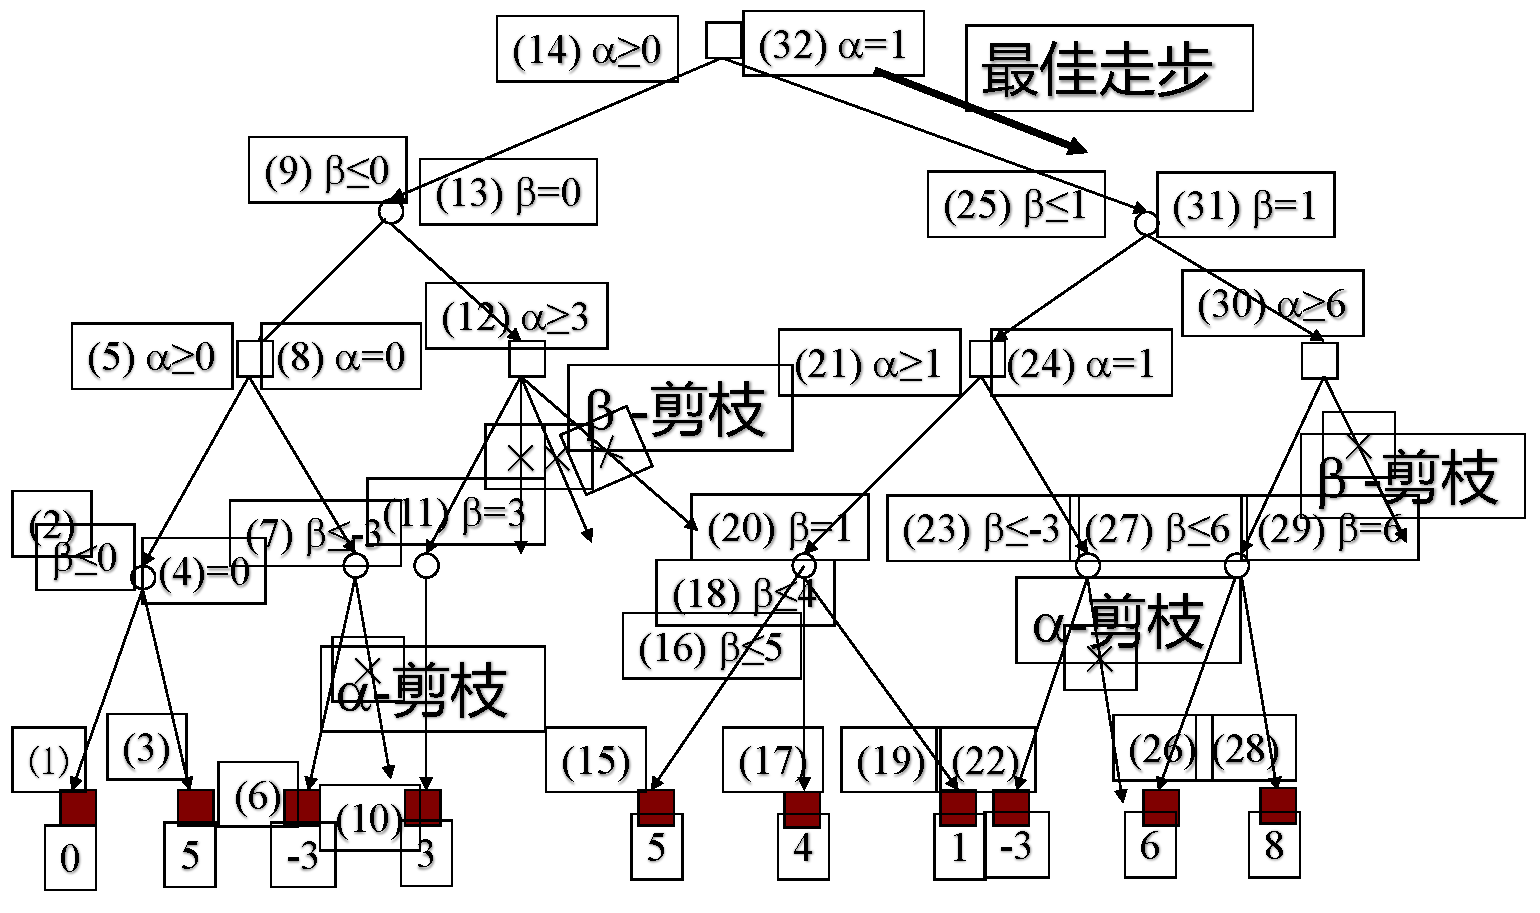
\includegraphics[width=\linewidth]{alpha-beta.pdf}

\section{高级搜索技术 (计算智能、群智能)}
% \begin{multicols}{2}
    组合优化问题
\begin{multicols}{2}
    遗传算法原理、操作:选择(轮盘赌算法)、交配、变异。

二进制编码交配方法:双亲双子法(某个点后面交换),变化交配法(如果亲代开头n个都一样,从第n个之后选),多交配位法 (好几组区间交换)

整数编码交配规则:常规交配法:选取一个交配位置,子代1交配位之前的基因选自父代1交配位之间的基因,交配位之后的基因,从父代2中按顺序选取那些没有出现过的基因.

父代1:1234|5678        子代1:1234|5786 \\
父代2:5217|3846        子代2:5217|3468

基于次序的交配法:首先在父代中随机地选定一组位置,从一父代中把该组位置上的数字依次取出;然后从另一父代中把所含的这些数字都暂时去掉(空位);最后按数字取出次序将另一父代的空位填充. 例如:

父代1: 1 2 3 4 5 6 7 8 9 10 \\
父代2: 5 9 2 4 6 1 10 7 3 8 \\
所选位置: 2,3,5,8 \\
子代1: 2 9 3 4 6 1 10 7 5 8
\end{multicols}
\clearpage
\begin{multicols}{2}
    基于位置的交配法:首先随机产生一组位置。对于这些位置上的基因,子代1从父代2中直接得到,子代1的其他位置的基因,按顺序从父代1中选取那些不相重的基因。子代2也类似处理。

父代1:1 2 3 4 5 6 7 8 9 \\
父代2:5 9 2 4 6 1 7 3 8 \\
选择:2,3,5,8 \\
子代1:1 9 2 4 6 5 7 3 8 \\
子代2: 9 2 3 4 5 6 1 8 7

基于部分映射的交配法:对于两个选定的父代染色体父代1和父代2,随机产生两个位置,两个父代在这两个位置之间的基因产生对应对,然后用这种对应对分别去替换两个父代的基因,从而产生两个子代。


父代1:2 6 4 3 8 1 5 7 9 \\
父代2:8 5 1 7 6 2 4 3 9 \\
选择$3 - 1$,即交换3,7;8,6;1,2; \\
子代1:1 8 4 7 6 2 5 3 9 \\
子代2:6 5 2 3 8 1 4 7 9



特点:随机搜索,对于指标函数没有要求,适用于并行求解。

蚁群算法:群智能搜索。信息素更新。

优点: 良好的鲁棒性、正反馈、及分布式并行计算等.

缺点: 迭代次数过多,尤其对城市数大于 100 的TSP问题.

易陷入局部最优,精度欠佳.
\end{multicols}
% \end{multicols}
% \vspace{-\baselineskip}
\section{谓词逻辑及其归结系统}

归结:反证法。将待证明的表达式转换为逻辑公式,进行归结。

归结原理就是从子句集S出发,应用归结推理规则导出子句集S1 ,再从S1出发导出S2 ,依次类推,直到某一个子句集Sn出现空子句为止.

根据不可满足性等价原理,若已知Sn为不可满足的,则可逆向依次推得S必为不可满足的.
用归结法证明定理,只涉及归结推理规则的应用问题,过程比较简单,因而便于实现机器证明. 

归结:设 C1 与 C2是子句集中的任意两个子句,如果C1中的文字L1与C2中的文字L2互补,那么从C1和C2中分别消去L1和L2,并将两个子句中的余下部分析取,构成一个新的子句C,这一过程称为归结.

\begin{multicols}{2}
    子句的要求:

\begin{outline}[citemize]
    \1 无量词约束
    \1 子句只是文字的析取$\lor$
    \1 否定符只作用于单个文字
    \1 子句间默认为合取$\land$
\end{outline}
\end{multicols}
\HRule
% \newcommand*{\lnot}{\sim}
% \newcommand*{\land}{\wedge}
% \newcommand*{\lor}{\vee}

\begin{multicols}{2}
标准化:
\begin{outline}[cenumerate]
    \1 消除蕴含符。$a \to b \Rightarrow \lnot a \lor b $

    \1 移动否定符。
        \2 $\lnot(a \land b) \Rightarrow \lnot a \land \lnot b $
        \2 $\lnot(a \lor b) \Rightarrow \lnot a \land \lnot b$
        \2 $\lnot(\exists x)P(x) \Rightarrow (\forall x)\lnot P(x)$
        \2 $\lnot(\forall x)P(x) \Rightarrow (\exists x)\lnot P(x)$
    
    \1 变量标准化:对于不同的约束,换名变量。
    \1 量词左移:移动存在和全称量词到最左边
    \1 消除存在量词(skolem化):如果左边没有全称量词,则换成常量,否则换成\emph{任意一个}全称量词限定的变量为因变量的函数。注意保留$\forall$
    \1 化为合取范式 (即$(a \lor b) \land (c \lor b)$)
    \1 隐去全称量词
    \1 表示为子句集:以逗号替代合取
    \1 \emph{变量换名}:每个子句用不同的变量。
\end{outline}
\end{multicols}
例子:
\begin{outline}[cenumerate]
    \1 $\forall x P(x) \to \paren*{\forall y \paren*{P(y) \to P(f(x, y))} \land \lnot \forall y \paren*{Q(x, y) \to P(y)}}$
    \1 $\bm{\lnot \forall x P(x)} \lor \paren*{\forall y \paren*{\bm{\lnot P(y) \lor} P(f(x, y))} \land \lnot \forall y \paren*{ \bm{\lnot Q(x, y) \lor } P(y)}}$
    \1 $\exists x \lnot P(x) \lor \paren*{\forall y \paren*{\lnot P(y) \lor P(f(x, y))} \land \exists y \paren*{Q(x, y) \land \lnot  P(y)}}$
    \1 $\exists x \lnot P(x) \lor \paren*{\forall y \paren*{\lnot P(y) \lor P(f(x, y))} \land \exists w \paren*{Q(x, w) \land \lnot  P(w)}}$
    \1 $\exists x \forall y \exists w \lnot P(x) \lor \paren*{\paren*{\lnot P(y) \lor P(f(x, y))} \land  \paren*{Q(x, w) \land \lnot  P(w)}}$
    \1 $\forall y \lnot P(a) \lor ((\lnot P(y) \lor P(f(a, y))) \land  Q(a, g(y)) \land \lnot  P(g(y)))$
    \1 $\forall y (\lnot P(a) \lor \lnot P(y) \lor P(f(a, y))) \land  (\lnot P(a) \lor Q(a, g(y))) \land  \lnot  (P(g(y)) \lor \lnot P(a))$
    \1 $(\lnot P(a) \lor \lnot P(y) \lor P(f(a, y))) \land  (\lnot P(a) \lor Q(a, g(y))) \land  (\lnot P(g(y)) \lor \lnot P(a))$
    \1 $(\lnot P(a) \lor \lnot P(y)\lor P(f(a, y))) ,\;  (\lnot P(a) \lor Q(a, g(y))) ,\; \\  (\lnot P(g(y)) \lor \lnot P(a))$
    \1 $(\lnot P(a) \lor \lnot P(y_1) \lor P(f(a, y_1))) ,\;  (\lnot P(a) \lor Q(a, g(y_2))) ,\; \\  (\lnot P(g(y_3)) \lor \lnot P(a))$
\end{outline}

谓词逻辑的归结:

归结式: 对于子句 C1$\lor$L1 和 C2$\lor$L2,如果L1 与 ~ L2 可合一,且 s 是其合一者,则(C1$\lor$C2)s 是其归结式.
例: P(x)$\lor$Q(y), $\lnot P(f(z)) \lor$R(z)
		   => Q(y)$\lor$R(z)      (s=f(z)/x)


置换:在谓词公式中用项 $t_i$ (常,变,函数)替换变量 $v_i$, 形如: 

$s = \set{t_1/v_1, t_2/v_2, \dots, t_n/v_n}$

对公式 E 实施置换 s 后得到的公式称为 E 的例,记作 E s.

可以结合,(E $s_1$) $s_2$  = E $s_1$ $s_2$,一般不可交换。

合一就是通过项对变量的置换,而使表达式(文字)一致. 若存在一个置换 s 使得表达式集{Ei}中每一个元素经置换后的例有:E1s =E2s= E3s=$\dots$,则称表达式集{Ei}是可合一的,这个置换 s 称作{Ei}的合一者.

例.$E_1 = \set{P(x, f(y), B), P(x, f(B), B)}, s = \set{A/x, B/y}$

$E\;s = \set{{P(A, f(B), B)}}$

如果 g 是公式集$\set{E_i}$的一个合一者,且对$\set{E_i}$的任意一个合一者s都存在一个置换$s'$,使得$s = g s'$,则称g为表达式{Ei}的最简单合一者mgu.

搜索策略:删除策略(删除无用字句)(纯文字删除法、重言式删除法、包孕删除法)、限制策略(通过设置选用条件对参与归结的子句进行限制,减少盲目性)(宽度优先、支持集、单元子句优先、线性输入形、祖先过滤形)

基于归结法的问题解答系统

先用谓词公式表示问题;证明目标公式是前提公式集的逻辑推论:如寻找Fido在哪儿,可以$\exists x, AT(Fido, x)$

先进行归结(反演树),证明结论的正确性;

用重言式($\exists x, AT(Fido, x) \lor \lnot AT(Fido, x)$)代替结论求反得到询问子句;

按照证明过程,进行归结;

最后,在原来为空的地方,得到的就是提取的回答.

修改后的证明树称为修改证明树.

例、if  Fido goes wherever John goes and if John is at school, where is Fido?

\begin{outline}[cenumerate]
    \1 前提:$(\forall x)(AT(John), x) \to AT(FIDO, x)$
        
        $AT(John, School)$
    \1 目标:$\exists AT(Fido, x)$
    \1 子句集: $\lnot AT(John, x_1) \lor AT(Fido, x_1)$% ~ AT(John, x1)  AT(Fido, x1), AT(John, School), ~ AT(Fido, x2)

        $AT(Jogn, School)$

        $\bm{\lnot AT(Fido, x_2)}$
\end{outline}

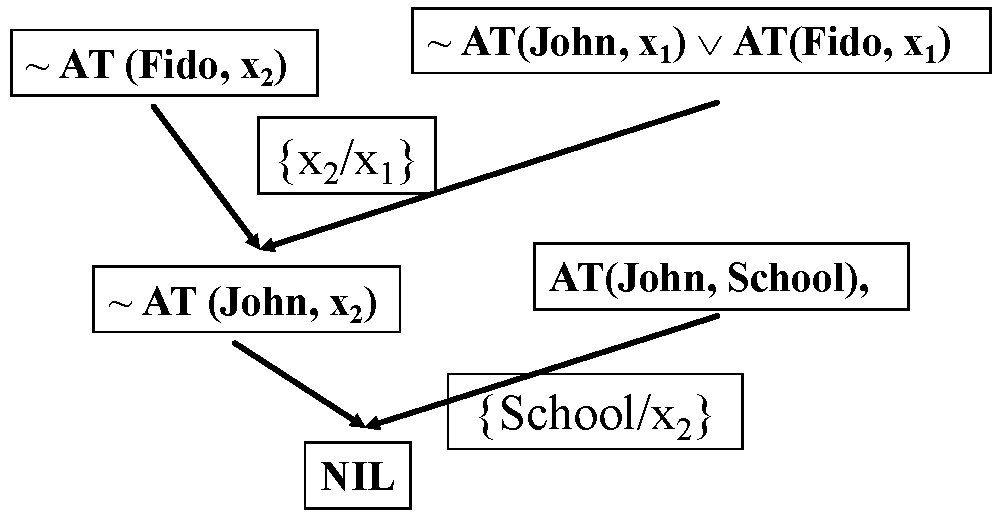
\includegraphics[width=0.5\linewidth]{stage1.pdf}
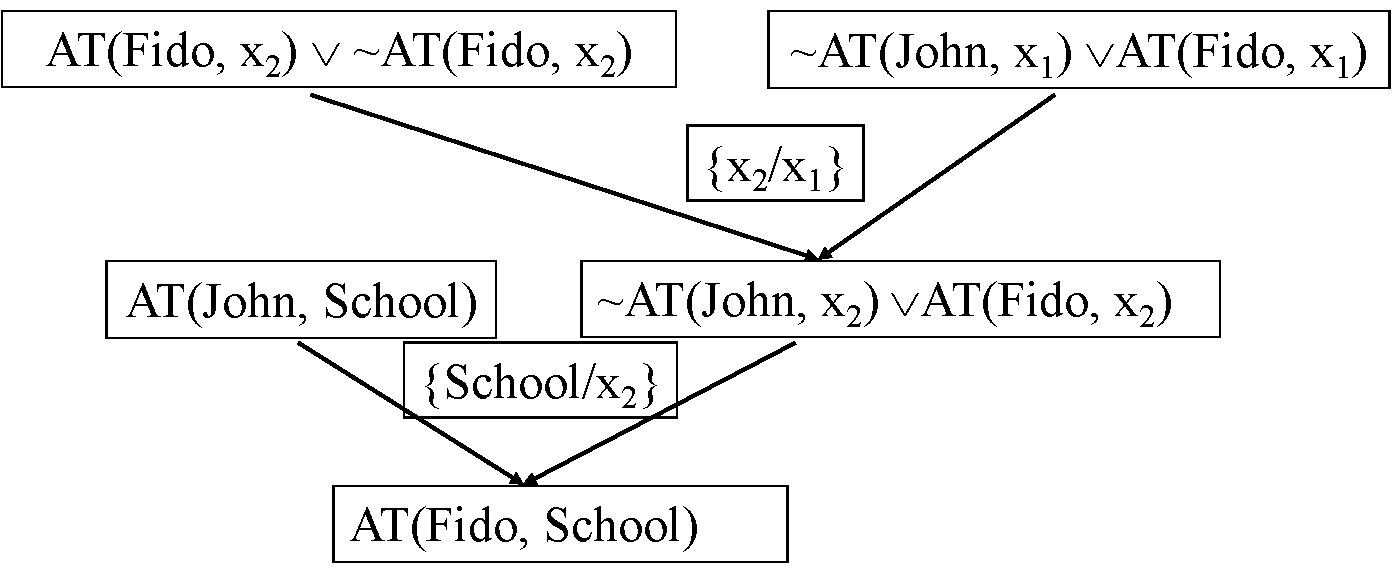
\includegraphics[width=0.5\linewidth]{stage2.pdf}


\vspace{-\baselineskip}

\section{知识表示}
研究知识的形式化方法,3种知识类型:

叙述型知识:有关系统状态、环境和条件,问题的概念、定义和事实的知识。

过程型知识:有关系统状态变化、问题求解过程的操作、演算和行动的知识。

控制型知识:有关如何选择相应的操作、演算和行动的比较、判断、管理和决策的知识。

从北京到上海,是乘飞机还是坐火车?叙述型:北京、上海、飞机、火车、时间、费用过程型:乘飞机、坐火车控制型:乘飞机较快、贵;坐火车较慢、便宜

同构变换:使问题更明确,便于求解;同构问题的解答等价于原始问题的解答。

同态变换:使问题更加简化,易于求解;原始问题有解,则同态问题有解,同态问题无解,则原始问题无解,它们之间是蕴涵关系。

\begin{multicols}{2}
    知识表示的方法:
\begin{outline}[citemize]
    \1 产生式系统
    \1 状态空间表示法、问题归约表示法(与或图)
    \1 谓词逻辑表示法
    \1 框架
    \1 面向对象的表示方法
    \1 \emph{语义网络}
    \1 基于XML 的表示法
    \1 本体表示法
    \1 知识图谱    
\end{outline}
\end{multicols}

语义网络的概念和特性\\
是一种采用网络形式表示人类知识的方法.\\
形式: 是带标识的有向图.\\
  节点: 表示物体、概念、事件、动作或态势,分为实例节点和类节点\\
  有向弧(也带有标识): 节点之间的语义联系,刻画节点之间的语义联系
\begin{outline}[citemize]
    \1 以个体为中心的语义联系:
        \2 ISA 表示类和实例之间的联系
        \2 AKO(a kind of) 表示类和父类的联系
        \2 part of 聚集联系:表示个体和组成成分(实例和实例)
        \2 属性链接:表示个体、属性和取值。用弧表示属性的label,指向的节点的value是属性的value
    \1 以谓词为重心的语义联系:
        \1 合取节点 AND
        \1 析取节点 OR
        \1 否定节点 可以直接用非+上述个体为中心的或引入非节点。
        \1 蕴含关系节点出发,一条弧指向命题的前提条件,记为ANKE,另一条弧指向该规则的结论,记为CONSE。
\end{outline}
分级网络: 引入一个类节点GS(对客观世界的一般性描述); 要表示的语句是GS的一个个体(实例)G, 如果G中含有n个全称变量, G在网络中有n+1条弧射出:
第一条:格式(FORM),它指向全称量词管辖的子网络(S1是一个特定的分割 A dog has bitten a postman)

后n条: $\forall$, 分别指向被全称量化的变量; 

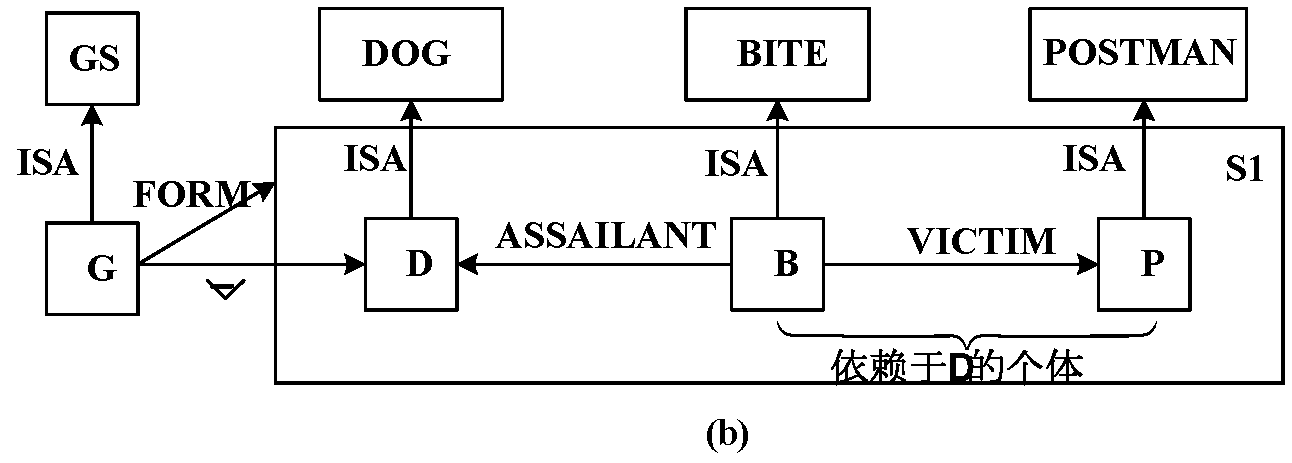
\includegraphics[width=\linewidth]{semantic_network.pdf}

\section{推理技术}
% \vspace{-\baselineskip}
\begin{multicols}{2}
    \begin{outline}[citemize]
        \1 事实表达式为与或形
        \1 规则形式:$L \to W$, 其中L为单文字
        \1 目标公式为文字析取
        \1 对事实和规则进行Skolem化,消去存在量词,变量受全称量词约束,对主合取元和规则中的变量换名
        \1 用“对偶形”对目标进行 Skolem 化,消去全称量词(用函数代替,$\forall y, y \to f(y)$),变量受存在量词约束,对析取元中的变量换名
        \1 事实表达成与或树,其中,$\land$对应树中“与”,$\lor$对应树中“或”
        \1 从事实出发,正向应用规则,到得到目标节点为结束的一致解图为止
        \1 存在合一复合时,则解图是一致的
    \end{outline}    
\end{multicols}
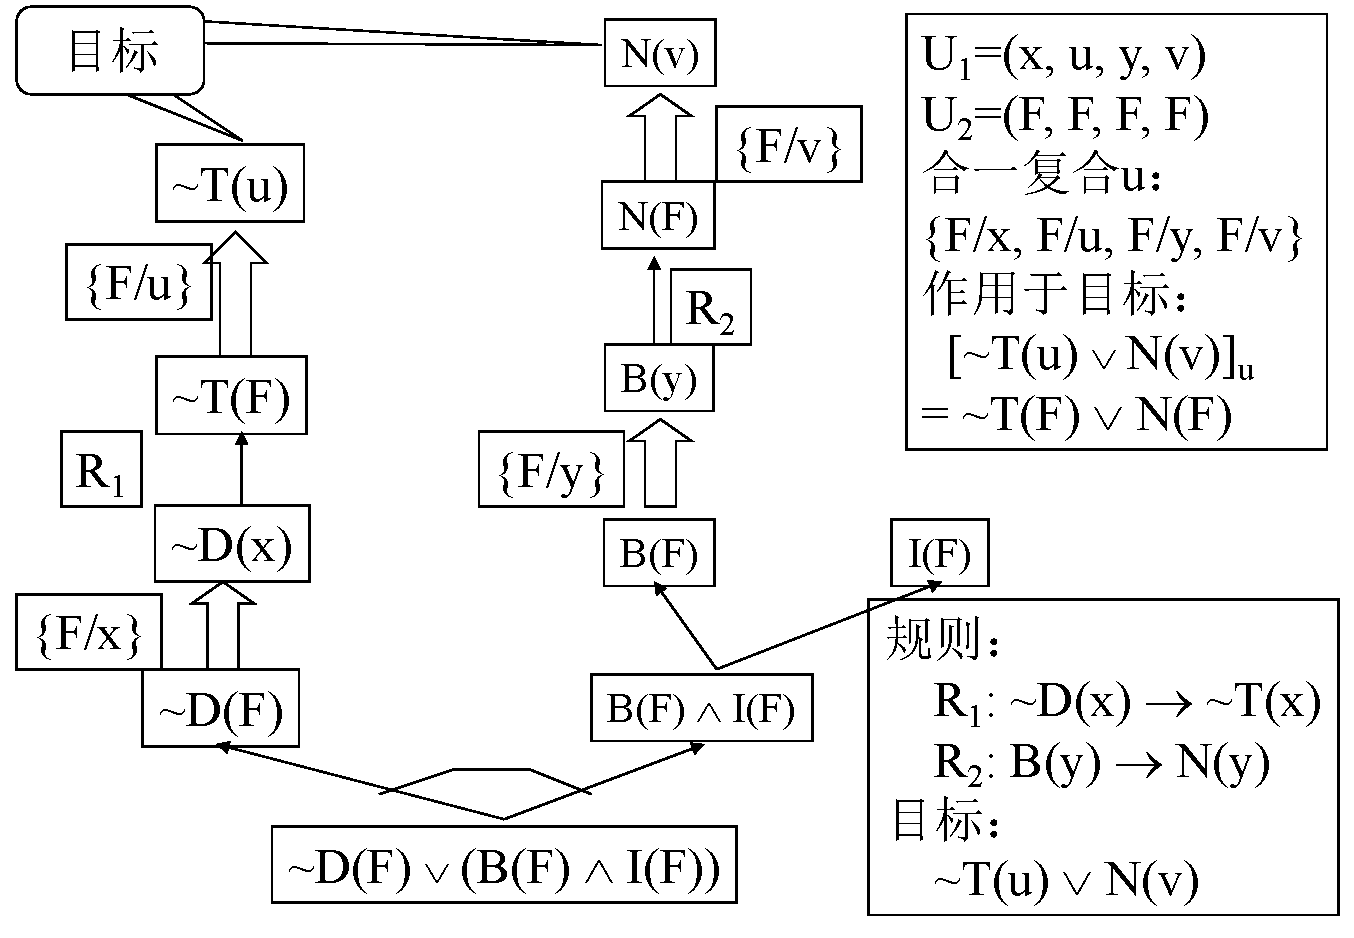
\includegraphics[width=\linewidth]{forward.pdf}
\HRule
逆向
\begin{multicols}{2}
    \begin{outline}[citemize]
        \1 目标为任意形的表达式
        \1 用“对偶形”对目标进行 Skolem化,即消去全称量词,变量受存在量词约束,对主析取元中的变量换名
        \1 目标用与或树表示,其中,“$\land$”对应树中“与”,“$\lor$”对应树中“或”
        \1 事实表达式是文字的合取
        \1 规则形式: L $\to$ W, 其中W为单文字,如形为:   	L$\to$ W1 $\land$W2,则变换为:      		        			L$\to$ W1 和 L$\to$ W2
        \1 从目标出发,逆向应用规则,到得到事实节点为结束条件的一致解图为止
    \end{outline}
\end{multicols}
\begin{center}
    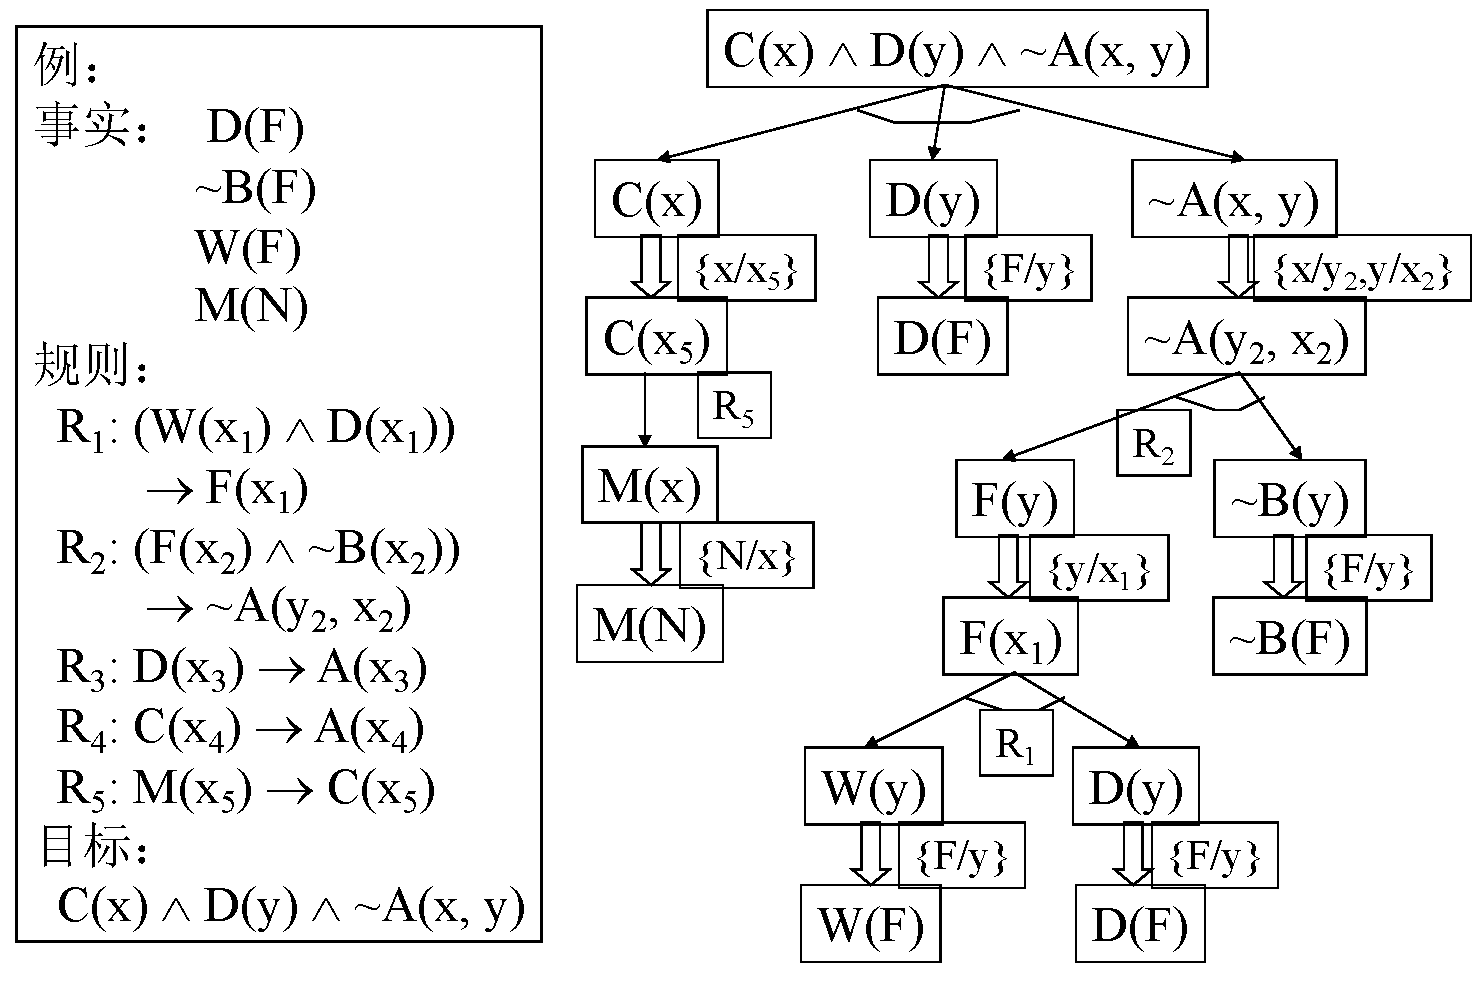
\includegraphics[width=.8\linewidth]{backward.pdf}
\end{center}

% 基于规则的演绎。正向,逆向。

\end{document}